 %%%%%%%%%%%%%%%%%%%%%%%%%%%%%%%%%%%%%%%%%%%%%%%%%%%%%%%%%%%%
%%  This Beamer template was created by Cameron Bracken.
%%  Anyone can freely use or modify it for any purpose
%%  without attribution.
%%
%%  Last Modified: January 9, 2009
%%
%%  http://cameron.bracken.bz/beamer-template

\documentclass[xcolor=x11names,compress]{beamer}

%% General document %%%%%%%%%%%%%%%%%%%%%%%%%%%%%%%%%%
\usepackage{graphicx}
\usepackage{tikz}
\usepackage{german}
\usetikzlibrary{decorations.fractals}
%%%%%%%%%%%%%%%%%%%%%%%%%%%%%%%%%%%%%%%%%%%%%%%%%%%%%
%\setbeameroption{show notes on second screen=left}

%% Beamer Layout %%%%%%%%%%%%%%%%%%%%%%%%%%%%%%%%%%
\useoutertheme[subsection=false,shadow]{miniframes}
\useinnertheme{default}
\setbeamertemplate{footline}{%
\begin{beamercolorbox}{section in head/foot}
    \color{gray}\vskip2pt~  \insertshorttitle\hfill\insertpagenumber{} %
    of \insertpresentationendpage{} ~\vskip2pt
\end{beamercolorbox}
}
\usefonttheme{serif}
\usepackage{palatino}

\setbeamerfont{title like}{shape=\scshape}
\setbeamerfont{frametitle}{shape=\scshape}

\setbeamercolor*{lower separation line head}{bg=DeepSkyBlue4} 
\setbeamercolor*{normal text}{fg=black,bg=white} 
\setbeamercolor*{alerted text}{fg=red} 
\setbeamercolor*{example text}{fg=black} 
\setbeamercolor*{structure}{fg=black} 
 
\setbeamercolor*{palette tertiary}{fg=black,bg=black!10} 
\setbeamercolor*{palette quaternary}{fg=black,bg=black!10} 

\renewcommand{\(}{\begin{columns}}
\renewcommand{\)}{\end{columns}}
\newcommand{\<}[1]{\begin{column}{#1}}
\renewcommand{\>}{\end{column}}
%%%%%%%%%%%%%%%%%%%%%%%%%%%%%%%%%%%%%%%%%%%%%%%%%%
\title[Secure Hash Algorithm]{Secure Hash Algorithm}



\begin{document}

%%%%%%%%%%%%%%%%%%%%%%%%%%%%%%%%%%%%%%%%%%%%%%%%%%%%%%
%%%%%%%%%%%%%%%%%%%%%%%%%%%%%%%%%%%%%%%%%%%%%%%%%%%%%%
\begin{frame}
\title{Secure Hash Algorithm}
%\subtitle{SUBTITLE}
\subtitle{SHA-256}
\author{
	Chi Trung Nguyen\\
	{\it T-Systems}\\
}
\date{
	\begin{tikzpicture}[decoration=Koch curve type 2] 
		\draw[DeepSkyBlue4] decorate{ decorate{ decorate{ (0,0) -- (3,0) }}}; 
	\end{tikzpicture}  
	\\
	\vspace{1cm}
	\today
}
\titlepage
\end{frame}

%%%%%%%%%%%%%%%%%%%%%%%%%%%%%%%%%%%%%%%%%%%%%%%%%%%%%%
%%%%%%%%%%%%%%%%%%%%%%%%%%%%%%%%%%%%%%%%%%%%%%%%%%%%%%
\begin{frame}{Inhalt}
%\tiny
\tableofcontents%[pausesections]
\end{frame}

%%%%%%%%%%%%%%%%%%%%%%%%%%%%%%%%%%%%%%%%%%%%%%%%%%%%%%
%%%%%%%%%%%%%%%%%%%%%%%%%%%%%%%%%%%%%%%%%%%%%%%%%%%%%%

\section{\scshape Einf"uhrung}
\subsection{Was ist ein Hash?}
\begin{frame}{Was ist ein Hash?}

\begin{itemize}
\item deutsch:  \glqq\textit{zerhacken}\grqq, \glqq \textit{verstreuen}\grqq
	\pause
\item Hashfunktion oder Streuwertfunktion erstellt aus beliebiger gro"ser Quellmenge eine immer gleich gro"se Zielmenge
\begin{itemize}
\item $ f(x) = f(x') $
	\pause
\end{itemize}
\item Einwegfunktion
\end{itemize}
\end{frame}

%%%%%%%%%%%%%%%%%%%%%%%%%%%%%%%%%%%%%%%%%%%%%%%%%%%%%%
%%%%%%%%%%%%%%%%%%%%%%%%%%%%%%%%%%%%%%%%%%%%%%%%%%%%%%

\section{\scshape Geschichte}
\subsection{SHA}
\begin{frame}{SHA Allgemein}
%The Secure Hash Algorithm is one of a number of cryptographic hash %functions published by the National Institute of Standards and Technology %(NIST) as a U.S. Federal Information Processing Standard (FIPS)
\begin{itemize}


%sha-0 wurde
\item 1993 vom {\bf National Institute of Standards(NIST)} 
als ein {\bf U.S. Federal Information Processing Standard (FIPS)} 
ver"offentlicht

	\pause
	%sha steht für secure hash algorithm und ist eine familie von hash algorithmn
\item Gruppe von kryptologischer Hashfunktionen
	\begin{itemize}
		\item SHA-0	
		\item SHA-1
		\item SHA-2
		\item SHA-3
	\end{itemize}

\end{itemize}
\end{frame}

%%%%%%%%%%%%%%%%%%%%%%%%%%%%%%%%%%%%%%%%%%%%%%%%%%%%%%
%%%%%%%%%%%%%%%%%%%%%%%%%%%%%%%%%%%%%%%%%%%%%%%%%%%%%%
\subsection{SHA-0}
\begin{frame}{SHA-0}
\begin{itemize}
\item 1993 ver"offentlicht
	\pause
	%ursprünglich als
\item Bestandteil des Digital Signature Algorithms (DSA) f"ur Digital Signature Standard (DSS) %empfohlen 1991

\end{itemize}
\end{frame}

%%%%%%%%%%%%%%%%%%%%%%%%%%%%%%%%%%%%%%%%%%%%%%%%%%%%%%
%%%%%%%%%%%%%%%%%%%%%%%%%%%%%%%%%%%%%%%%%%%%%%%%%%%%%%
\subsection{SHA-1}
\begin{frame}{SHA-1}
\begin{itemize}
\item 1995 ver"offentlicht
\pause
\item aufgrund Designfehler in SHA-0
%es wurde ein rechtsshift durch ein linksshift ersetzt
\end{itemize}
\end{frame}


%%%%%%%%%%%%%%%%%%%%%%%%%%%%%%%%%%%%%%%%%%%%%%%%%%%%%%
%%%%%%%%%%%%%%%%%%%%%%%%%%%%%%%%%%%%%%%%%%%%%%%%%%%%%%
\subsection{SHA-2}
\begin{frame}{SHA-2}
\begin{itemize}
\item 2002 ver"offentlicht
\pause
\item existiert in mehreren Bit Variante
%%die hier gelistet sind(nächste folie)

%%TODO
%%MERKLE DEMGARD
%%EVENTUELL UNTERSCHIEDE ZU SHA0 und SHA1


\end{itemize}
\end{frame}

%%%%%%%%%%%%%%%%%%%%%%%%%%%%%%%%%%%%%%%%%%%%%%%%%%%%%%
%%%%%%%%%%%%%%%%%%%%%%%%%%%%%%%%%%%%%%%%%%%%%%%%%%%%%%
\begin{frame}[shrink=30]{}
\begin{table}[c]
\caption{Secure Hash Algorithmus Eigenschaften}
\begin{tabular}[ht]{|c|p{0.2\textwidth}|p{0.2\textwidth}|p{0.2\textwidth}|p{0.2\textwidth}|}
  \hline
  Algorithmus &  Message Gr"o"se(bits) & Block Gr"o"se(bits) & Word Gr"o"se(bits) & Message Digest Gr"o"se(bits)\\
  \hline\hline
  SHA-1   & $<2^{64}$  &  512 & 32 & 160\\
  SHA-224 & $<2^{64}$  &  512 & 32 & 224\\
  SHA-256 & $<2^{64}$  &  512 & 32 & 256\\
  SHA-384 & $<2^{128}$ & 1024 & 64 & 384\\  
  SHA-512 & $<2^{128}$ & 1024 & 64 & 512\\  
  \hline
\end{tabular}
\label{tab:meinetabelle}
\end{table}
\end{frame}


%%%%%%%%%%%%%%%%%%%%%%%%%%%%%%%%%%%%%%%%%%%%%%%%%%%%%%
%%%%%%%%%%%%%%%%%%%%%%%%%%%%%%%%%%%%%%%%%%%%%%%%%%%%%%
\section{\scshape Implementierung}
\subsection{Algorithmus}
\begin{frame}{Funktionen}
$ Ch(E,F,G) = (E\wedge F) \oplus (\neg E\wedge G)$
$ Maj(A,B,C) = (A\wedge B) \oplus (A\wedge C) \oplus (B\wedge C)$\\
$ \Sigma_0 = (A\ggg 2) \oplus (A\ggg 13) \oplus (A\ggg 22) $\\
$ \Sigma_1 = (A\ggg 6) \oplus (A\ggg 11) \oplus (A\ggg 25) $\\
\end{frame}


%%%%%%%%%%%%%%%%%%%%%%%%%%%%%%%%%%%%%%%%%%%%%%%%%%%%%%
%%%%%%%%%%%%%%%%%%%%%%%%%%%%%%%%%%%%%%%%%%%%%%%%%%%%%%
\begin{frame}{Darstellung des Algorithmus}
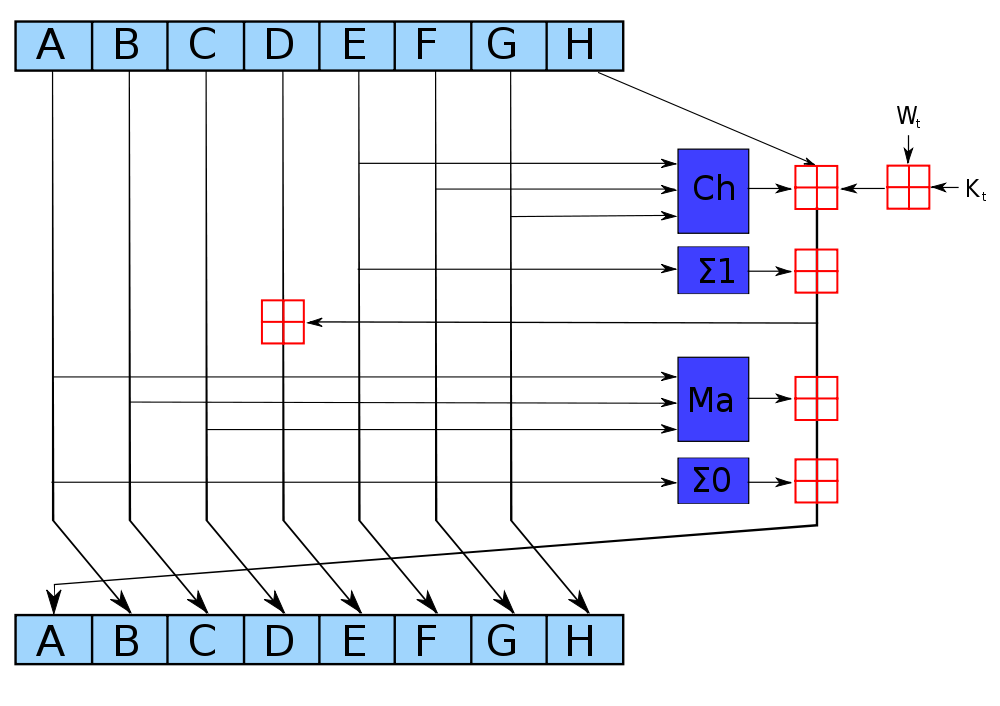
\includegraphics[scale=0.3]{sha256.png}\\
\end{frame}


%%%%%%%%%%%%%%%%%%%%%%%%%%%%%%%%%%%%%%%%%%%%%%%%%%%%%%
%%%%%%%%%%%%%%%%%%%%%%%%%%%%%%%%%%%%%%%%%%%%%%%%%%%%%%
\subsection{Pseudocode}
\begin{frame}{Pseudocode}
\begin{itemize}
\item Initialize variables
(first 32 bits of the fractional parts of the square roots of the first 8 primes 2..19):\\
\texttt{h[0..7] := 0x6a09e667,[...],0x5be0cd19}
\pause
\item Initialize table of round constants
(first 32 bits of the fractional parts of the cube roots of the first 64 primes 2..311):\\
\texttt{k[0..63] := 0x428a2f98,[...], 0xc67178f2}
\end{itemize}



\end{frame}
%%%%%%%%%%%%%%%%%%%%%%%%%%%%%%%%%%%%%%%%%%%%%%%%%%%%%%
%%%%%%%%%%%%%%%%%%%%%%%%%%%%%%%%%%%%%%%%%%%%%%%%%%%%%%

\begin{frame}{Preprocessing}
\begin{itemize}
\item \texttt{bit $1$ zur $message$ hinzuf"ugen} \pause
\item \texttt{anzahl von $k$ bits $0$ hinzuf"ugen, wobei $k$ die kleinst m"ogliche Zahl >= 0, so dass die L"ange der $message$ (in bits) Modulo 512 minus 64 bits ist} \pause
\item \texttt{L"ange der $message$(vor dem Preprocessing), in bits, als 64-bit big-endian integer hinzufügen}\newline \newline \pause
\item \texttt{$message$ in 512-bit chunks teilen}
\item \texttt{foreach chunk\{}\newline
    \texttt{teile chunk in sechzehn 32-bit big-endian Worte $w[0..15]$}
\end{itemize}




\end{frame}
%%%%%%%%%%%%%%%%%%%%%%%%%%%%%%%%%%%%%%%%%%%%%%%%%%%%%%
%%%%%%%%%%%%%%%%%%%%%%%%%%%%%%%%%%%%%%%%%%%%%%%%%%%%%%

\begin{frame}{Erweiterung der Worte}

\begin{itemize}

\item[]
\texttt{for $i=16$ to $63$ \{}
		 \begin{itemize}
		 \item[] $s0$ := ($w[i-15]$ rightrotate $7$) xor ($w[i-15]$ rightrotate $18$) xor ($w[i-15]$ rightshift $3$) \newline
        \item[] $s1$ := ($w[i-2]$ rightrotate $17$) xor ($w[i-2]$ rightrotate $19$) xor ($w[i-2]$ rightshift $10$) \newline
        \item[] $w[i]$ := $w[i-16]$ + $s0$ + $w[i-7]$ + $s1$ \newline \}
		 \end{itemize}
		 %%aufschreiben was ist rechtsrotate,was ist rechtsshift + was ist das padding(?) erklären können!
         
\end{itemize}


\end{frame}
%%%%%%%%%%%%%%%%%%%%%%%%%%%%%%%%%%%%%%%%%%%%%%%%%%%%%%
%%%%%%%%%%%%%%%%%%%%%%%%%%%%%%%%%%%%%%%%%%%%%%%%%%%%%%

\begin{frame}{Hashzuweisung}
\texttt{$a := h0$ \\
    $b := h1$ \\
    $c := h2$ \\
    $d := h3$ \\
    $e := h4$ \\
    $f := h5$ \\
    $g := h6$ \\
    $h := h7$} 
%%h0 = nachkommastelle der quadratwurzel
\end{frame}
%%%%%%%%%%%%%%%%%%%%%%%%%%%%%%%%%%%%%%%%%%%%%%%%%%%%%%
%%%%%%%%%%%%%%%%%%%%%%%%%%%%%%%%%%%%%%%%%%%%%%%%%%%%%%

\begin{frame}{Hauptschleife}
\begin{itemize}[]
\item[]
\texttt{for $i=0$ to $63$ \{} \\
\begin{itemize}[]
\item[]
    \texttt{$S0$ := ($a$ rightrotate $2$) xor ($a$ rightrotate $13$) xor ($a$ rightrotate $22$)} \pause 
\item[]
	\texttt{$maj$ := ($a$ and $b$) xor ($a$ and $c$) xor ($b$ and $c$)}\pause 
\item[]
	\texttt{$t2$ := $S0$ + $maj$} \pause
\item[]
	\texttt{$S1$ := ($e$ rightrotate $6$) xor ($e$ rightrotate $11$) xor ($e$ rightrotate $25$)} \pause
\item[]
	\texttt{$ch$ := ($e$ and $f$) xor ((not $e$) and $g$)} \pause
\item[]
	\texttt{$t1$ := $h$ + $S1$ + $ch$ + $k[i]$ + $w[i]$} \pause
\item[]
        $h$ := $g$ \\
        $g$ := $f$ \\
        $f$ := $e$ \\
        $e$ := $d$ + $t1$ \\
        $d$ := $c$ \\
        $c$ := $b$ \\
        $b$ := $a$ \\
        $a$ := $t1$ + $t2$
\end{itemize}

\end{itemize}

\end{frame}
%%%%%%%%%%%%%%%%%%%%%%%%%%%%%%%%%%%%%%%%%%%%%%%%%%%%%%
%%%%%%%%%%%%%%%%%%%%%%%%%%%%%%%%%%%%%%%%%%%%%%%%%%%%%%

\begin{frame}{Hauptschleife}
\texttt{$h0$ := $h0$ + $a$ \\
    $h1$ := $h1$ + $b$ \\
    $h2$ := $h2$ + $c$ \\
    $h3$ := $h3$ + $d$ \\
    $h4$ := $h4$ + $e$ \\
    $h5$ := $h5$ + $f$ \\
    $h6$ := $h6$ + $g$ \\
    $h7$ := $h7$ + $h$} \newline \} \newline \} $//Ende$ $der$ $foreach$-$Schleife$
\end{frame}
%%%%%%%%%%%%%%%%%%%%%%%%%%%%%%%%%%%%%%%%%%%%%%%%%%%%%%
%%%%%%%%%%%%%%%%%%%%%%%%%%%%%%%%%%%%%%%%%%%%%%%%%%%%%%

\begin{frame}{Ausgabe}
\texttt{digest = hash = $h0$ append $h1$ append $h2$ append $h3$ append $h4$ append $h5$ append $h6$ append $h7$}
\end{frame}
%%%%%%%%%%%%%%%%%%%%%%%%%%%%%%%%%%%%%%%%%%%%%%%%%%%%%%
%%%%%%%%%%%%%%%%%%%%%%%%%%%%%%%%%%%%%%%%%%%%%%%%%%%%%%
\section{\scshape Anwendung}
\subsection{Verwendungszweck}
\begin{frame}{Verwendungszweck}

\begin{itemize}
\item Digitale Zertifikate und Signaturen 
	\pause
\item Passwortverschl"usselung
\begin{itemize}
	\item pam\textunderscore unix: sha2, md5
	\item htpasswd(Apache): sha1, md5
	\item MySQL: sha1
\end{itemize}
\pause
\item Pr"ufsummen bei Downloads
\end{itemize}


\end{frame}
%%%%%%%%%%%%%%%%%%%%%%%%%%%%%%%%%%%%%%%%%%%%%%%%%%%%%%
%%%%%%%%%%%%%%%%%%%%%%%%%%%%%%%%%%%%%%%%%%%%%%%%%%%%%%
\subsection{Sicherheitsl"ucken}
\begin{frame}{Sicherheitsl"ucken \& Angriffsvektoren}

\end{frame}

%%%%%%%%%%%%%%%%%%%%%%%%%%%%%%%%%%%%%%%%%%%%%%%%%%%%%%
%%%%%%%%%%%%%%%%%%%%%%%%%%%%%%%%%%%%%%%%%%%%%%%%%%%%%%
\section{\scshape Ausblick}
\subsection{SHA-3}
\begin{frame}{SHA-3}

\end{frame}



\end{document}